\documentclass{article}
\usepackage{graphicx}
\title{Dynamical Systems}
\author{Harsha Ravula}

\begin{document}
\maketitle
\newpage
\tableofcontents
\newpage
\section{What is a Dynamical System?}
\subsection{Introduction}
A dynamical system is a guide to the evolution of variables and their outcomes over a certain period of time. There are two main streams of dynamical systems.
First, we have continuous time systems which can be represented by 
\linebreak
\newline
\begin{center}
    \textsc{$y' = f(y,t)$}   
 \end{center}
where $y = y(t)$. 
\newline
\linebreak
Another type of dynamical system is the discrete time dynamical systems, but here we will be looking into continuous time systems.
\subsection{Importance of dynamical systems}
Dynamical systems are used to evaluate the change in variables in numerous fields and disciplines across the professional world. These models are used in financial and economic forecasting, environmental modeling, medical diagnosis, industrial equipment diagnosis, and a host of other applications. 
\newline
\linebreak
The majority of applications fall into three categories. First we have the predictive category, where the objective of constructing systems is to predict future states of the variables over a specific amount time. This is achieved by scrutinizing the behavior of the system over its past and present states, then successively building a model which accounts for the past and present behavior of the system. Secondly, we have the diagnostic category, in which the objective is to infer what possible past states of the system have led to the current state and observe any possible correlations. Lastly, the final category is where the objective is neither to predict the future nor explore the past but rather to draw conclusions for what has occurred in the system.  
\newline
\linebreak
An example of the predictive category, consider a chemist studying the chemical reactions between two compounds. He creates a system of differential equations which take into account the temperature, pressure, and moles of compounds. From here the scientist can input the control variables such as the temperature, pressure, and moles and examine the behavior of the system. If the system deems to be accurate then the scientist can use the system to examine the multitude of possible outcomes by simply solving the system. 
\newline
\linebreak
Although this example is somewhat unexciting to the masses, dynamical systems can be used to predict numerous situations. One of the more famous applications is modeling the spread of HIV virus and predicting the number of people becoming infected at some point into the future. We can use systems to predict virus spread and ultimately mitigate the contamination rate. 
\section{Qualitative Properties of a Dynamical System}
Now we ask the question what would we like to know about the dynamical system?
\newline
\linebreak
Firstly we are would like to find the fixed points. A fixed point is a point that does not change upon application of a system of differential equations. In particular, a fixed point of a function is equal to itself. That is $f(x) = x$ then $x$ is a fixed point.
\newline
\linebreak
Fixed points also represent a point to which the system converges or diverges to or from respectively. A stable fixed point is one that attracts where as  a unstable fixed points repels.  Here is a pictoral representation.
\begin{figure}[ht!]
\centering
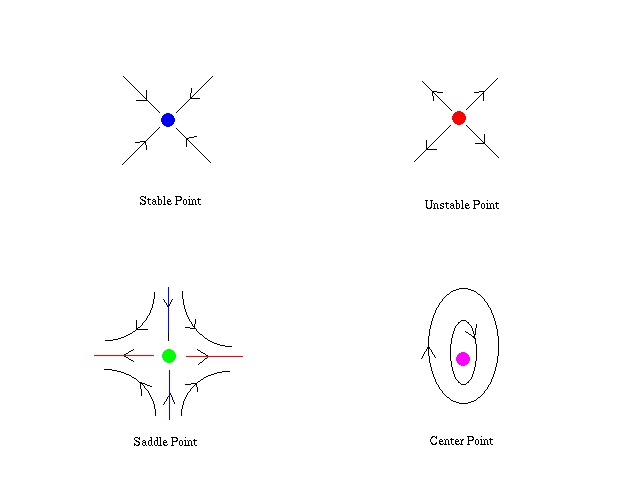
\includegraphics[width=90mm]{points.jpg}
\caption{Types of Fixed Points}
\label{overflow}
\end{figure}
\newline
Each fixed point has its own orientation, meaning the way in which the fixed point attracts of repels. 
These are classified into
\newline
\linebreak
1) Unstable – node (Top right)
\newline
2) Unstable spiral
\newline
3) Semi-stable (star or degenerate node)
\newline
4) Stable Node (Top left)
\newline
5) Stable Spiral
\newline
6) Stable Center (Bottom right)
\newline
7) Unstable Saddle Point (Bottom left)
\newpage

The next qualitative property we would like to know are the basins of attraction, a basin of attraction is the region in which any initial condition located in that region converges to a corresponding fixed point. We can find the basins of attracting by plotting a vector field of the dynamical system. The arrows in the vector field point to the direction that an initial condition follows if located in that position. And having knowledge of the direction can give us insight into the behavior and to what might happen over a period of time. Here is a 3-D plot of some basins of attraction for a system.

\begin{figure}[ht!]
\centering
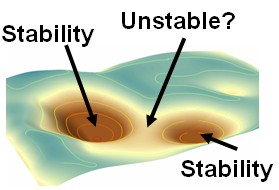
\includegraphics[width=60mm]{boa.jpg}
\caption{Basins of attraction}
\label{overflow}
\end{figure}
The last qualitative property that we are going to discuss is the trajectory of initial conditions. This is for a given initial condition, i.e. the starting point of a system given by a coordinate point (x,y), where will the initial points converge or diverge to. This is crucial when studying a dynamical system. Refer back to our chemistry example, when the chemist adds 20 moles of chemical A and 50 moles of chemical B the path of the trajectory of the initial condition will tell us where the reaction will end up, or in other words how much product will be formed and in how much time. Here is an example of what a trajectory of an initial point looks like. The blue line represents the path of the initial condition.
\begin{figure}[ht!]
\centering
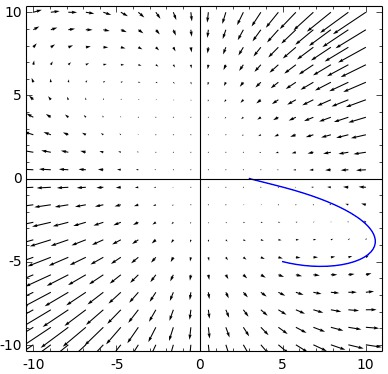
\includegraphics[width=45mm]{traj.jpg}
\caption{Trajectory of an Initial Condition}
\label{overflow}
\end{figure}
\newpage
\section{An Example Dynamical System}
\subsection{Briefing of the example}
Now, lets take a look at a very important dynamical system. 
\linebreak
\newline
\begin{center}
    \textsc{$\frac{dS}{dt} = - \beta  SI +  \mu (N-S) +  \gamma I$}   
\end{center}
\begin{center}
    \textsc{$ \frac{dI}{dt} = \beta  SI -  \mu I -  \gamma I$} 
\end{center}
Where:
\linebreak
\newline
$S(t)$ is used to represent the number of individuals not yet infected with the disease at time t
\newline
\linebreak
$I(t)$ denotes the number of individuals who have been infected with the disease and are capable of spreading the disease
\newline
\linebreak
$\beta$ is the Contact rate
\newline
\linebreak
$\mu$ is the Average death rate
\newline
\linebreak
$N$ is the Total Population
\newline
\linebreak
$\gamma$ represents the mean recovery/death rate or $1/\gamma$ is the the mean infective period
\newline
\linebreak
This model as inferred from the terminology depicts the dynamics of the disease infection rate of an epidemic. This is a famous model which is referred to as the SIS model.
\newline
\linebreak
Now from here our main question is how do we extract information from this system. Firstly, assuming that we have done our research regarding the population and statistics of the virus we can input values for coefficients and constants respectively.
\newline
\linebreak
Let us take $\beta = .05$ which means there is a 1 in 20 chance that you contract the disease from somebody else, and $\mu = .5$ which means that about half the people that contract the disease pass away. Also we can assume that we are in a small tribe of people and the total population is about $N = 50$ members. And Lastly we let $\gamma = .9$ which means that there are 9 recoveries to every death.
\newpage
\subsection{Solution to the example}
In order to completely find the qualitative solution to the system we must calculate the fixed points, find the stability of each fixed point, calculate the orientation of each fixed point, find the basins of attraction after plotting the vector field of the system. And finally draw the trajectory of the initial condition.
\newline
\linebreak
The analyze function I have written allows us to completely understand the dynamical system at hand. We will solve the given example using the analyze function.
 First when we run the analyze function we are greeted with an interactive gui, which easily allows us to input the $x'$ and $y'$ function as well as the desired initial points. Let us input the initial values corresponding to the given equations and constants above and choose 5 initial infected humans and 45 susceptible humans.
\begin{figure}[ht!]
\centering
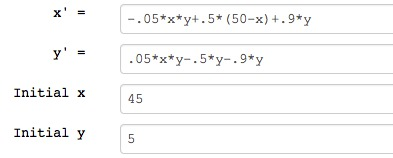
\includegraphics[width=60mm]{initialentryr.jpg}
\caption{Initial Entry}
\label{overflow}
\end{figure}
\newline
We press enter and the solutions are draw and posted right below the input box. For this example we are given:
\begin{figure}[ht!]
\centering
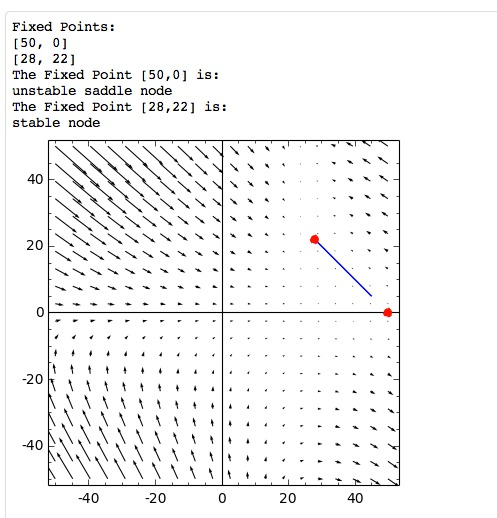
\includegraphics[width=70mm]{results.jpg}
\caption{The results}
\label{overflow}
\end{figure}
\newline
Finally, let us interpret the results.
\newline
Firstly, we see that the system has two fixed points  [50,0] and [28,22] which are represented by red circles on the vector field. Next we can observe that the [50,0] fixed point is an unstable saddle node and the [28,22] fixed point is a stable node. 
\newline
\linebreak
What do these mean? 
\newline
\linebreak
This means that the system converges to the [28,22] fixed point which translates to the population of 50 members will end up with 22 infected people and 28 healthy people over a fixed period of time assuming that we have atleast one infected human in the population. This is supported by us observing that the graph has a blue line that converges to the red dot located at [28,22]. Changing the control variables $N,\beta,\gamma,$and $\mu$ will yield a different fixed point or in common terms a different number of infected and healthy people within the same population of 50. Changing the number of initial infected and healthy people will result in a longer or shorter time of convergence to the stable fixed point located at [28,22], we can easily do this by changing the number inside the inital $x$ and inital $y$ boxes.
In conclusion, we see that the system converges to about 22 infected human beings. From here we try implement vaccinations and other medical practices to change the control variables, such as reducing the contact rate. This example illustrates the importance of the information we can extract from any given system by finding all the qualitative attributes of the system.
\newpage
\section{References}
\begin{quote}
1. Deconinck, Bernard. "Dynamical Systems and Chaos An Introduction." . Department of Applied Mathematics University of Washington, 9 Apr. 2009. Web. 17 May 2014. <http://faculty.washington.edu/joelzy/402notesbernard.pdf>.
\end{quote}

\begin{quote}
2."Introduction to Learning Dynamical Systems." Introduction to Learning Dynamical Systems. N.p., n.d. Web. 19 May 2014. <http://cs.brown.edu/research/ai/dynamics/tutorial/Documents/DynamicalSystems.html>.
\end{quote}
\begin{quote}
3. "Epidemic model." Wikipedia. Wikimedia Foundation, 25 May 2014. Web. 27 May 2014. <http://en.wikipedia.org/wiki/Epidemicmodel>.
\end{quote}
\end{document}
